\documentclass[main]{subfiles}

\begin{document}
\begin{lect} {2019-09-25}
	\hsubsubsection{2.9.4}{Теорема о непр. диф. отобр. в точке}
	U - откр (всегда)
	\begin{Theorem}[о непр. диф. в точке]
		\[a \in U \subset \R^n, \q f: U \ra \R^m\]
		\[f \text{ - непр. диф. в точке a}\]
		Тогда:
		\begin{enumerate}
			\item f - непр в некоторой окр. т. а
			\item f - диф-ма в т. а
		\end{enumerate}
	\end{Theorem}

	\begin{proof}[m=1]
		\begin{enumerate}
			\item f - непр диф в точке a $\lra$ все ч.п. опр. в $V_a$ и непр в т.а.\\
			      Из лок св-ва непр ф-ий $\Ra$ $\e$ окр $V_a(\delta):$ все ч.п. огр. конст $M>0$
			      \[|\dfrac{\d f}{\d x_k}(x)|<M \q \forall x \in V_a(\delta)\]
			      \[|f(x+h)+f(x)| \os{\text{лемма}}{=} \sum\limits_{k=1}^n \dfrac{\d f}{\d x_k} (c^k) h_k| \leqslant \sum\limits_{k=1}^n |\dfrac{\d f}{\d x_k} (c^k)| |h_k| \leqslant\]
			      \[\leq M \sum\limits_{k=1}^n |h_k| \leqslant M n ||h||,\]
			      если $||h|| \ra 0$ $\Ra$ $|f(x+h)-f(x)| \ra 0$
			\item Докажем, что f - диф-ма в т. а\\
			      Т.к. все ч.п. непр. в т. а
			      \[\Ra \forall E>0\q \e \delta_1,\delta_2,...,\delta_n>0\]
			      \[||x-a|| < \delta_k \RA \Abs{\dfrac{\d f}{\d x_k}(x)-\dfrac{\d f}{\d x_k}(a)} < \dfrac{\E}{\sqrt n}\]
			      Возьмем $\delta=min_{1 \leqslant k \leqslant n} \delta_k$
			      \[\letus h: a + h \in V_a(\delta)\]
			      \begin{figure}[h!]
				      \center{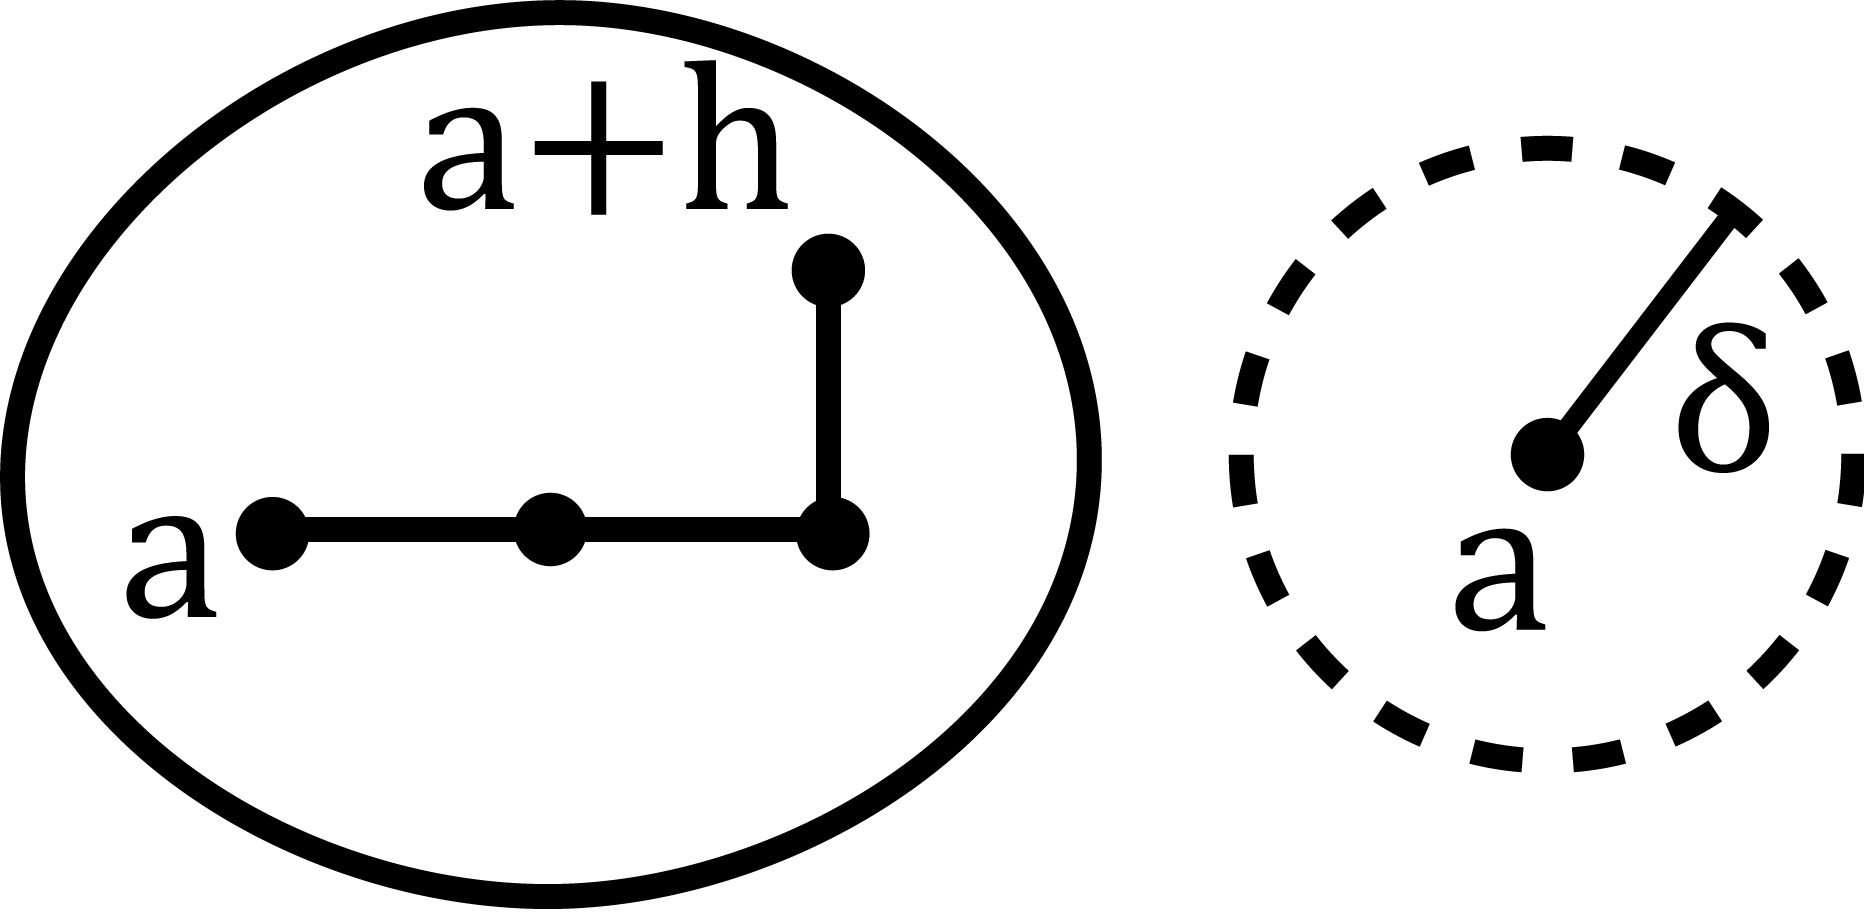
\includegraphics[width = 4cm]{pics/5_1}}
			      \end{figure}
			      По лемме $\e C^k (\in V_a(\delta))$:
			      \[f(a+h)-f(a) = \sum_{k=1}^n \dfrac{\d f}{\d x_k}(C^k)h_k =\]
			      \[= \sum_{k=1}^n \dfrac{\d f}{\d x_k}(a) h_k + \sum_{k=1}^n \left[\dfrac{\d f}{\d x_k}(c^k) - \dfrac{\d f}{\d x_k}(a)\right]h_k\]
			      Правое слагаемое - $R(h)$. Надо доказать, что $R(h)=o(h)\q h \ra 0$
			      \[||R(h)|| \leqslant \sum_{k=1}^n \abs{\dfrac{\d f}{\d x_k}(c^k)-\dfrac{\d f}{\d x_k}(a)} \cdot |h_k| \leqslant \text{(КБШ)}\]
			      \[\leqslant \sqrt{\sum_{k=1}^n \Abs{\dfrac{\d f}{\d x_k}(c^k)-\dfrac{\d f}{\d x_k}(a)}^2} \cdot ||h|| \leqslant \E ||h||\]
			      т.к. $\dfrac{\d f}{\d x_k}$ - непр. в т. а и $c^k \in V_a(\delta)$
			      \[\Ra |\dfrac{\d f}{\d x_k}(c^k)-\dfrac{\d f}{\d x_k}(a)|<\dfrac{\E}{\sqrt{n}}\]
			      \[\forall \E>0\q \e \delta: ||h|| < \delta \Ra \dfrac{R(h)}{||h||}<\E\]
			      т.е. $R(h)=o(||h||)$, $h \ra 0 \RA f$ - диф в т. а
		\end{enumerate}
	\end{proof}

	\hsubsubsection{2.9.5}{Теорема о хар-ке непр. диф. отобр.}
	\begin{Theorem}[хар-ка непр. диф. отобр.]
		\[a \in U \subset \R^n\]
		\[f \in C^1(U) \lra f: U \ra R^m  \text{ - диф-ма на U},\q d.f \in C(U;\LL(\R^n,R^m))\]
		\[d.f \in C(U;\LL(\R^n,R^m)) \LRA\]
		\[\LRA \forall \E > 0 \q \e \delta > 0: \forall a,b \in U: \Abs{a-b} < \delta \Ra \Abs{d_a f - d_b f} < \E\]
	\end{Theorem}

	\begin{proof}
		($\Ra$):
		\[||d_a f - d_b f|| \leqslant ||d_a f - d_b f ||_{\HS}
			= \sqrt{\sum_{j=1}^n \sum_{k=1}^n \abs{\dfrac{\d f}{\d x_k}(a) - \dfrac{\d f}{\d x_k}(b)}^2} \us{a \ra b}{\ra} 0\]
		($\La$):
		\[\text{Пусть мы знаем, что }df \in C(U, \LL(|\R^n, \R^m|)\]
		\[\Abs{\dfrac{\d f}{\d x_k}(a)-\dfrac{\d f}{\d x_k}(b)} = || d_a f(e^k)-d_a f(e^k)|| = ||(d_a f =d_b f)(x_k)|| \leqslant\]
		Напоминание: $||f||-норм$, $||Ax \leqslant ||A||*||x||$
		\[\leqslant ||d_a f - d_b f ||* 1 \us{a \ra b}{\ra} 0 \text{ - норма оператора}\]
		\[df \in C(U,\LL(\R^n,R^m))\]
	\end{proof}

	\subsection{Частные производные высших порядков}
	\begin{examples}
		\begin{enumerate}
			\item $f(x,y)=X^y$
			      \[f'_x=y x^{y-1}\]
			      \[f'_y=x^y \ln x\]
			      \[\dfrac{\d}{\d y} \Br{\dfrac{\d f}{\d x}}=\dfrac{\d^2 f}{\d y \d x}=(y x^{y-1})'_y=x^{y-1}+y x^{y-1} \ln x\]
			      \[\dfrac{\d}{\d x} \Br{\dfrac{\d f}{\d y}}=\dfrac{\d^2}{\d x \d y}=(x^y \ln x)'_x=y x^{y-1} \ln x + x^y \dfrac{1}{x}\]
			\item $f(x,y)=x y g(x,y)$
			      \[f'_x (0,y)=\lim_{x \ra 0} \dfrac{f(x,y)-f(0,y)}{x}=\lim_{x \ra 0}  \dfrac{x y g(x,y)}{x} = \lim_{x \ra 0} y g(x,y)\]
			      \[f'_y(x,0)=\lim_{y \ra 0} x g(x,y)\]
			      \[\dfrac{\d^2 f}{\d y \d x} (0,0)= \lim_{y \ra 0}  \dfrac{f'_x(0,y)-f'_x(0,0)}{y}=\lim_{y \ra 0} \lim_{x \ra 0}  g(x,y) \]
			      \[\dfrac{\d^2 f}{\d x \d y}= \lim_{x \ra 0} \lim_{y \ra 0} g(x,y)\]
			      Возьмем, например,
			      \[g(x,y) = \begin{cases}
					      \dfrac{x^2-y^2}{x^2+y^2}, & (x,y) \neq (0,0) \\
					      0,                        & (x,y) = (0,0)
				      \end{cases}\]
			      \[\lim_{x \ra 0} \lim_{y \ra 0} g \neq \lim_{y \ra 0} \lim_{x \ra 0} g \Ra f''_{x y}(0,0) \neq f''_{y x}(0,0)\]
		\end{enumerate}
	\end{examples}

	\begin{Definition}
		\[f: U \ra \R^m \q a \in U \subset \R^n\]
		Пусть для $r \in N$ определены ч.п. f порядка r в окрестности точки а
		\[\dfrac{\d^{r+1} f}{\d x_{i_1} ... \d x_{i_{r+1}}} := \dfra{\d}{\d x_{i_{r+1}}}(\dfrac{\d^r}{\d x_{i_r}...\d x_{i_1}})\]
		\[i_k \in \{1,...,n\}\]
	\end{Definition}

	\subsubsection{Теорема о замене порядка диф-ия в ч.п.}
	\begin{Theorem}
		\[f: U \ra \R^m, \q a \in U \subset \R^n\]
		\[\text{Пусть }\dfrac{\d f}{\d x_j},\q \dfrac{\d f}{\d x_k},\q \dfrac{\d^2 f}{\d x_j \d x_k}\]
		\[\text{И } \dfrac{\d^2 f}{\d x_j \d x_k} \text{ - непр. в т. а}\]
		\[\text{Тогда }\e \dfrac{\d^2 f}{\d x_k \d x_j} (a) \text{ и } \dfrac{\d^2 f}{\d x_k \d x_j} (a) = \dfrac{\d^2 f}{\d x_j \d x_k}(a)\]
	\end{Theorem}

	\begin{Proof}
		\[x_k=x,\q x_j=y\]
		\[\dfrac{\d^2 f}{\d x \d y} \text{ - непр. в т. }a=(a_1;a_2)\]
		\begin{figure}[h!]
			\center{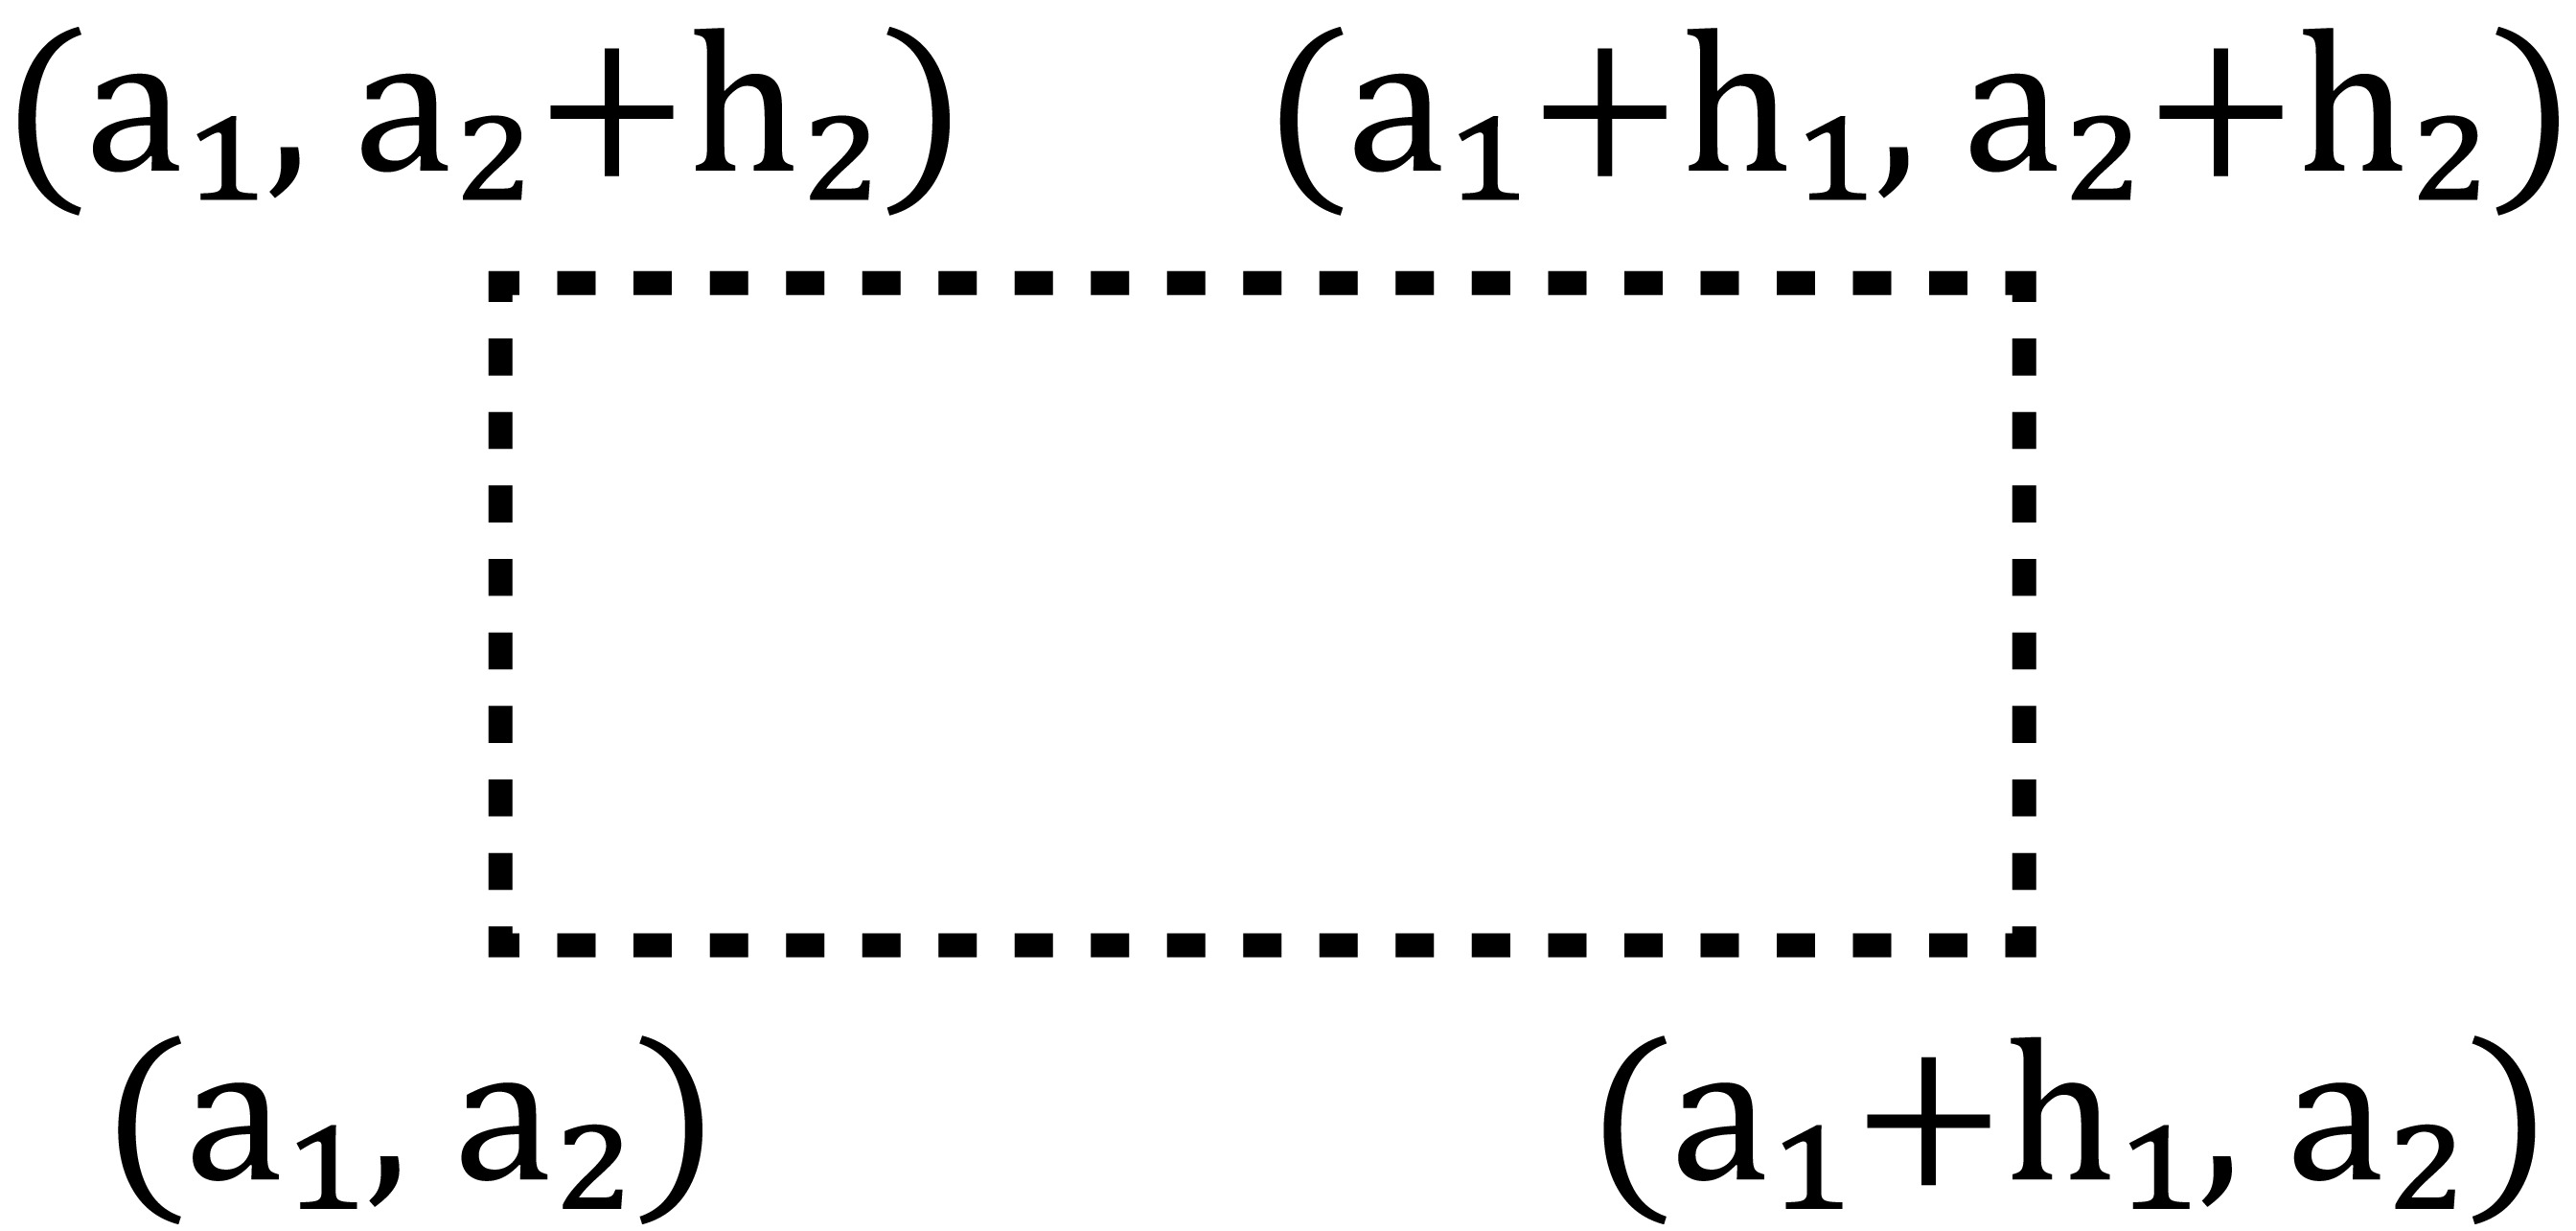
\includegraphics[width = 5cm]{pics/5_2}}
		\end{figure}
		\[h \text{ - приращение, } a+h \in V_a\]
		\[\varphi(x):=f(x;a_2+h_2)-f(x,a_2) \text{ - диф-ма}\]
		по т. Лагранжа $\e \xi:$
		\[\varphi(a_1+h_1)-\varphi(a_1)=\varphi'(\xi)h_1 \q a_1 < \xi<a_1+h\]
		\[\varphi(a_1+h_1)-\varphi(a_1) = f_{11}-f_{10}-f_{01}+f_{00} = h_1 \Br{\dfrac{\d f}{\d x}(\xi,a_2+h_2)-\dfrac{\d f}{\d x}(\xi,a_2)}=\]
		\[\os{\text{по т. Лагранжа}}{\us{\e \eta: a_2 < \eta<a_2+h}{=}} h_1 \dfrac{\d^2 f}{\d y \d x}(\xi, \eta) h_2\]
		\[\Abs{\us{\frac{\d^2 f}{\d y \d x}(\xi,\eta)}{\dfrac{f_{11}-f_{10}-f_{01}+f_{00}}{h_1 h_2}}-\dfrac{d^2 f}{\d y \d x}(a_1,a_2)}<\E\q (*)\]
		т.к. $\dfrac{d^2 f}{\d y \d x}$ - непр. в т. а $\e \delta>0: ||h||<\delta \Ra (*) < \E$
		\[\text{В}\q (*)\q h_2 \ra 0\]
		\[\dfrac{f_{11}-d_{10}}{h_2} \ra \dfrac{\d f}{\d g}(a_1+h_1, a_2)\]
		\[\dfrac{f_{01}-f_{00}}{h_2} \ra \dfrac{\d f}{\d y}(a_1,a_2)\]
		\[\Abs{\dfrac{1}{h_1}(\dfrac{\d f}{\d y}(a_1+h_1,a_2)-\dfrac{\d f}{\d y}(a_1,a_2))}\]
		\[\Ra \lim_{h \ra 0} \dfrac{\dfrac{\d f}{\d y}(a_1+h_1,a_2)-\dfrac{\d f}{\d y}(a_1,a_2)}{h_1}=\dfrac{\d^2 f}{\d y \d x}(a_1,a_2)\]
		Левая часть = $\dfrac{d^2 f}{\d x \d y}(a_1,a_2)$
	\end{Proof}

	\begin{Definition}
		\[f \in C^k(U), \text{ если $\e$ и непр. ч.п. порядка k}\]
		\[C^{\infty}(U)=\cup_{k \in \N} C^k (U)\]
	\end{Definition}

	\begin{consequence}
		Если $f \in C^k(U)$, то $\dfrac{\d^k f}{\d x_{i_1} ... \d x_{i_k}}$ не зависит от порядка диф-ия
	\end{consequence}

	\subsubsection{Формула Тейлора}
	\begin{Theorem}
		\[f \in C^{m+1}(U) \q p \in U \q [p;p+h] \subset U\]
		\[\varphi(t):=f(p+th) \q 0 \leqslant t \leqslant 1\]
		\[\gamma(t)=p+th\]
		\[\varphi(t)=(f \circ \gamma)(t) \in C^{m+1}[0,1]\]
		\[\varphi(t)=\sum_{k=0}^m \dfrac{\varphi^{k}(0)}{k!}t^k + R_{m+1}(t, \varphi)\]
		\[f(p+h)=\varphi(1)=\sum_{k=0}^m \dfrac{\varphi^k(0)}{k!}+R_m(1, \varphi)\]
		\[\varphi(t)=f(\varphi+th)\]
		\[\varphi'(t)=\sum_{j=0}^n \dfrac{\d f}{\d x_j}(p+th)h_j\]
		\[\varphi''(t)=\sum_{j=0}^n (\dfrac{\d f}{\d x_j} (p+th))'_t h_j = \sum_{j=0}^n h \sum_{k=1}^n \dfrac{\d f}{\d x_k \d x_j}(p+th)h_k = \sum_{j,k=1}^n \dfrac{\d^2 f}{\d x_k x_j}(p+th) h_k h_j\]
		\[\varphi^{(k)}(t) = \sum_{j_1,j_2,...,j_k}^n \dfrac{\d^k f}{\d x_{j_1}...\d x_{j_k}}(p+th)h_{j_1}...h_{j_k}\]
		\[\varphi^{(k)}=\sum_{j_1,...,j_k=1}^n \dfrac{\d^k f}{\d x_{j_1}... \d x_{j_k}}(p) h_{j_1}...h_{j_k} -\text{k-линейная форма (от $h_{j_1}...h_{j_k}$)}\]
		\[f(p+h)=\sum_{k=0}^m \dfrac{1}{k!} \sum_{j_1,...,j_k=1}^n \dfrac{\d^k f}{\d x_{j_1}... \d x_{j_k}}(p) h_{j_1}...h_{j_k}+R_{m+1}\]
		\[R_{m+1}=\dfrac{1}{(n+1)!} \varphi^{(n+1)}_{0 < ]xi <1} (\xi) 1=\dfrac{1}{(n+1)!} \sum_{j_1,...,j_k}^n \dfrac{\d^{n+1} f}{\d x_{j_1}...\d x_{j_{n+1}}} (p+\xi_k) h_{j_1}...h_{j_k} \]
		\[d^k_p f(h):=\sum_{j_1,...,j_k=1}^n \dfrac{\d^k f}{\d x_{j_1}...\d x_{j_k}}(p) h_{j_1}...h_{j_k}\]
		\[f(p+h)=\sum_{k=1}^m \dfrac{1}{k!} d_p^k f(h)+R_{m+1}\]
	\end{Theorem}

	\begin{Example}
		\[f(x,y)=x^3+x y^2 \q p=(1,-1) \q \d f;\d^2 f - ?\]
		\[\dfrac{\d f}{\d x}=3x^2+y^2\]
		\[\dfrac{\d f}{\d y}=2x y\]
		\[d_p f(h)=(4;-2) \begin{pmatrix} %круглая матрица!
				h_1 \\ h_2
			\end{pmatrix}=4h_1-2h_2\]
		\[\dfrac{\d^2 f}{\d x^2}=6x\]
		\[\dfrac{\d^2 f}{\d x \d y}=2y=\dfrac{\d^2 f}{\d y \d x}\]
		\[\dfrac{\d^2 f}{\d y^2}=2x\]
		\[d_p^2 f(h)=\dfrac{\d^2 f}{\d x^2} h_1^2+\dfrac{\d^2 f}{\d x \d y} h_1 h_2 + \dfrac{d^2 f}{\d x \d y} h_2 h_1 + \dfrac{\d^2 f}{\d y^2} h_2^2 =\]
		\[= \dfrac{\d^2 f}{\d x^2} h_1^2 + 2 \dfrac{\d^2 f}{\d x \d y}h_1 h_2+\dfrac{\d^2 f}{\d y^2} h_2^2=6h_1^2+4h_1 h_2 2 h_2^2 \text{ - квадр. форма}\]
		\[d_p^k f (\us{приращение арг. (вместо h)}{dx})=(\sum_{j=1}^n \dfrac{\d}{\d x_j} d x_j)^k f\]
		\[d^3_p f \begin{pmatrix} %круглая
				dx \\ dy
			\end{pmatrix}=(\dfrac{\d}{\d x} + \dfrac{\d}{\d y} dy)^3=\]
		\[f(x,y)=\dfrac{\d^3 f}{\d x^3} d^3 x + 3 \dfrac{\d^3 f}{\d x^2 \d y} d x^2 dy+3 \dfrac{\d^3 f}{\d x \d y^2}dx dy^2+\dfrac{\d^3 f}{\d y^3}dy^3 \]
	\end{Example}

	\subsubsection{Оценка остаточного члена в форме Лагранжа}

	\[M_{m+1}:=\sup_U \max \Abs{\dfrac{\d^{m+1} f}{\d x_{j_1}...x_{j_{m+1}}}(x)}\]
	\[|R_{m+1}| \leqslant \dfrac{M_{m+1}}{(m+1)!} \sum_{j_1,...j_{m+1}=1}^n |h_{j_1}| |h_{j_{m+1}}|= \dfrac{M_{m+1}}{(m+1)!}(\sum_{j=1}^n |h_j|)^{m+1} \leqslant \dfrac{M_{m+1}}{(m+1)!}(\sqrt{n}||h||)^{m+1}\]
	Если $M_m \leqslant C^m * m! \Ra$ в некоторой окр. т. p ряд Тейлора сх. равномерно (и абсолютно)

	\begin{Theorem}[остаточный член в форме Пеано]
		\[f \in C^m (U)\]
		\[T_m(f;p,h)=\sum_{k=0}^m \dfrac{1}{k!} \sum_{j_1...j_k}^n \dfrac{\d^k f}{\d x_{j_1} \d x_{j_k}} (h_{j_1}...h_{j_k})\]
		\[\text{Тогда } f(p+h)=T_m(f;p,h)=o(||h||^m) \q h \ra 0\]
	\end{Theorem}

	\begin{Proof}
		\[f(p+h)-T_m(f;p,h)=R_m\]
		Докажем потом!
	\end{Proof}

	\subsubsection{Локальный экстремум}
	\[f: U \ra \R^1,\q U \subset \R^m\]
	Было: f - диф. в т. $a\in U$. a - лок экстр. $\Ra \nabla_a f=0$

	(необх. условие экстр.)

	\begin{definition}
		$a\in U$ назыв. критической для f, если $d_a f=0$
	\end{definition}

	a - лок. экстр. f - диф-ма в а $\Ra$ а - кр. т. f

	Из ф. Тейлора (а - крит. точка):
	\[f(a+h)=f(a)+\sum_{j=1}^n \us{=0 т.к. точка крит.}{\dfrac{\d f}{\d x_j}(a)} h_j+\dfrac{1}{2} \sum_{i,j=1}^n \dfrac{\d^2 f}{\d x_i \d x_j}(a) h_i h_j+o(||h||^2)\]

	\begin{Definition}
		\[K(h)=\sum_{i,j=1}^n a_{i j} h_i h_j; \q a_{i j}=i j\]
		К - положительно определенная кв. форма, если:
		\[K(h)>0$ $\forall h \neq 0\]
		Отрицательно опредеенная, если:
		\[K(h)<0$ $\forall h \neq 0\]
		Неопределенная, если:
		\[\e h_1,k: K(h)>0,\q K(k)<0\]
		Полуопределнная, если:
		\[\e h \neq 0 \qq P(h) < 0\]
	\end{Definition}

	\subsubsection{Критерий Cильвестра}
	K - положительно опр $\lra$
	\[\Delta_1=a_{1 1}>0\]
	\[\Delta_2=\begin{vmatrix} %там были круглые матрицы, тут квадратные
			a_{11} & a_{12} \\
			a_{21} & a_{22}
		\end{vmatrix}\]
	\[\Delta_k>0\]
	\[\Delta_k=\begin{vmatrix}
			a_{11} & ... & a_{1k} \\
			...    & ... & ...    \\
			a_{k1} & ... & a_{kk}
		\end{vmatrix}\]

	K-отрицательно определена, если $(-1)^k \Delta_k>0$

	\begin{Theorem}[дост. условие лок. экстремума]
		\[f: U \ra \R^1 \q f \in C^2(U), \q a \in U\]
		a - крит. т. f, тогда:
		\begin{enumerate}
			\item $d_a^2 f$ - положит. опр. $\Ra$ a - лок. min
			\item $d_a^2 f$ - отриц. опр. $\Ra$ a - лок. max
			\item $d_a^2 f$ - неопр. $\Ra$ a - не лок. экстр.
		\end{enumerate}
	\end{Theorem}

	\begin{Example}
		\[d(x,y) - x^4 - 2x^2 + y^4\]
		Критическая т.:
		\[\begin{cases}
				f'_x=4x^3-4x=0 & (0,\ 0) \text{ - т. сгущ.} \\
				f'_y=4y^3=0    & (1,\ 0)\q (-1,\ 0)
			\end{cases}\]
		\[f''_{xx} = 12 x^2 - 4\]
		\[f''_{xy} = 0\]
		\[f''_{yy} = 12 y^2\]
		\begin{tabular}{ccc}
			(0, 0) & (0, 0) & (-1, 0) \\
			\hline
			-4     & 8      & 8       \\
			0      & 0      & 0       \\
			0      & 0      & 0
		\end{tabular}
		\[d^2_{(0,\ 0)} f = - 4 dx^2\]
		\[d^2_{(1,\ 0)} f = 8 dx^2\]
		\[\Delta_1 = -4 \q \Delta_2 = 0 \text{ - теор. не раб.}\]
		\[f(x,\ y) = (x^2 - 1)^2 + y^2 - 1\]
		\[f(\pm 1,\ 0) = -1 \text{ - глоб min}\]
		\[f(0,\ \delta) = 1 + \delta^4 - 1 > 0\]
		\[f(\sigma,\ 0) = (\sigma^2 - 1)^2 + 0 - 1 < 0\]
	\end{Example}
\end{lect}
\end{document}
